\section{Optuna results}
\label{sec:optuna}

\subsection{Feedforward Neural Network}

\begin{figure}[!ht]
    \centering 
    \caption{
        Optuna exploration on FNN hyperparameters. 
        Objective value corresponds to error rate on validation set across all classes.
    }
    \label{fig:optuna_fnn}
    \begin{subfigure}{.32\textwidth}
        \centering 
        \caption{}
        
\includegraphics[width=\linewidth]{../../python_code/plots/fnn/contour.pdf}
    \end{subfigure}
    \begin{subfigure}{.32\textwidth}
        \centering 
        \caption{}
        
\includegraphics[width=\linewidth]{../../python_code/plots/fnn/optimization_history.pdf}
    \end{subfigure}
    %
    \begin{subfigure}{.32\textwidth}
        \centering 
        \caption{}
        
\includegraphics[width=\linewidth]{../../python_code/plots/fnn/param_importances.pdf}
    \end{subfigure}
    \begin{subfigure}{.32\textwidth}
        \centering 
        \caption{}
        
\includegraphics[width=\linewidth]{../../python_code/plots/fnn/rank.pdf}
    \end{subfigure}
    %
    \begin{subfigure}{.32\textwidth}
        \centering 
        \caption{}
        
\includegraphics[width=\linewidth]{../../python_code/plots/fnn/slice.pdf}
    \end{subfigure}
    \begin{subfigure}{.32\textwidth}
        \centering 
        \caption{}
        
\includegraphics[width=\linewidth]{../../python_code/plots/fnn/terminator_improvement.pdf}
    \end{subfigure}
\end{figure}

\clearpage
\subsection{Decision Tree}

\begin{figure}[!ht]
    \centering 
    \caption{
        Optuna exploration on DT hyperparameters. 
        Objective value corresponds to error rate on validation set across all classes.
    }
    \label{fig:optuna_dt}
    \begin{subfigure}{.32\textwidth}
        \centering 
        \caption{}
        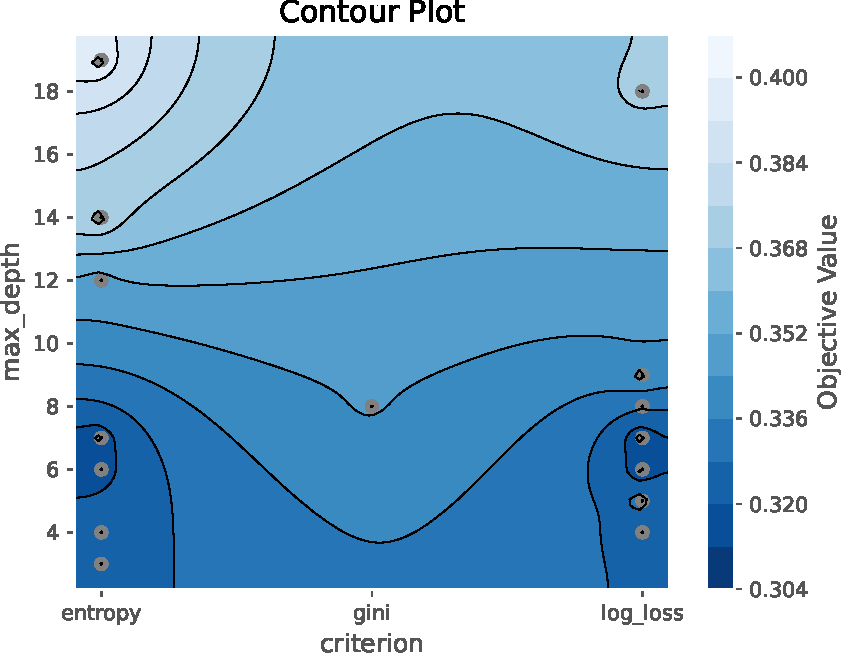
\includegraphics[width=\linewidth]{../../python_code/plots/dt/contour.pdf}
    \end{subfigure}
    \begin{subfigure}{.32\textwidth}
        \centering 
        \caption{}
        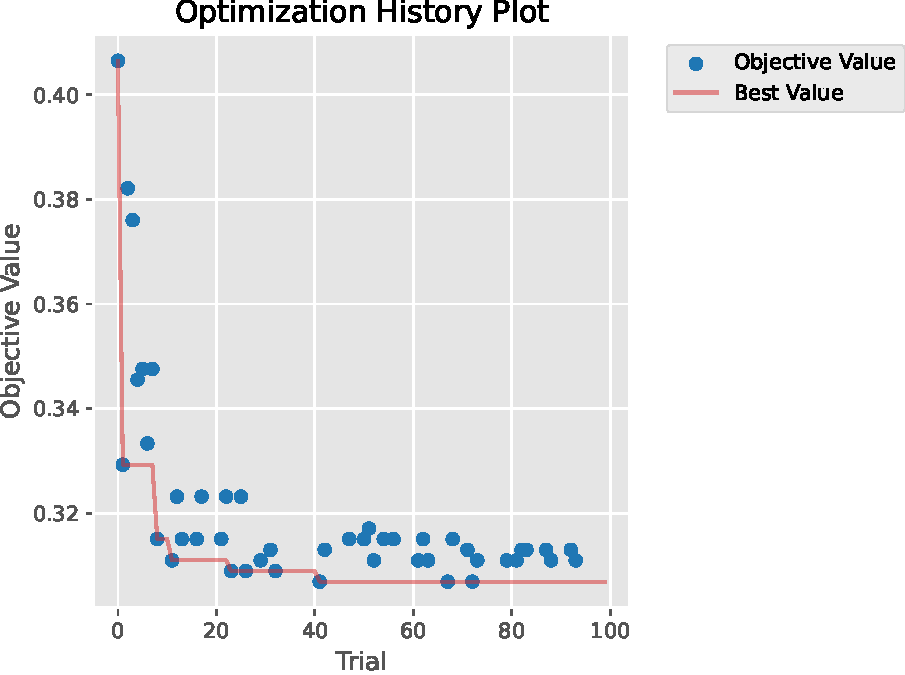
\includegraphics[width=\linewidth]{../../python_code/plots/dt/optimization_history.pdf}
    \end{subfigure}
    %
    \begin{subfigure}{.32\textwidth}
        \centering 
        \caption{}
        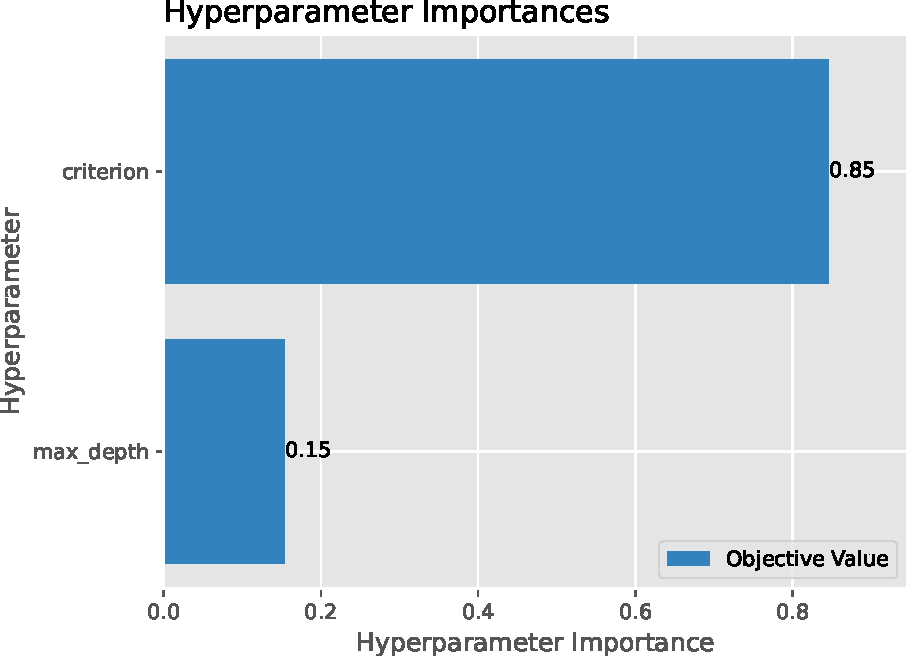
\includegraphics[width=\linewidth]{../../python_code/plots/dt/param_importances.pdf}
    \end{subfigure}
    \begin{subfigure}{.32\textwidth}
        \centering 
        \caption{}
        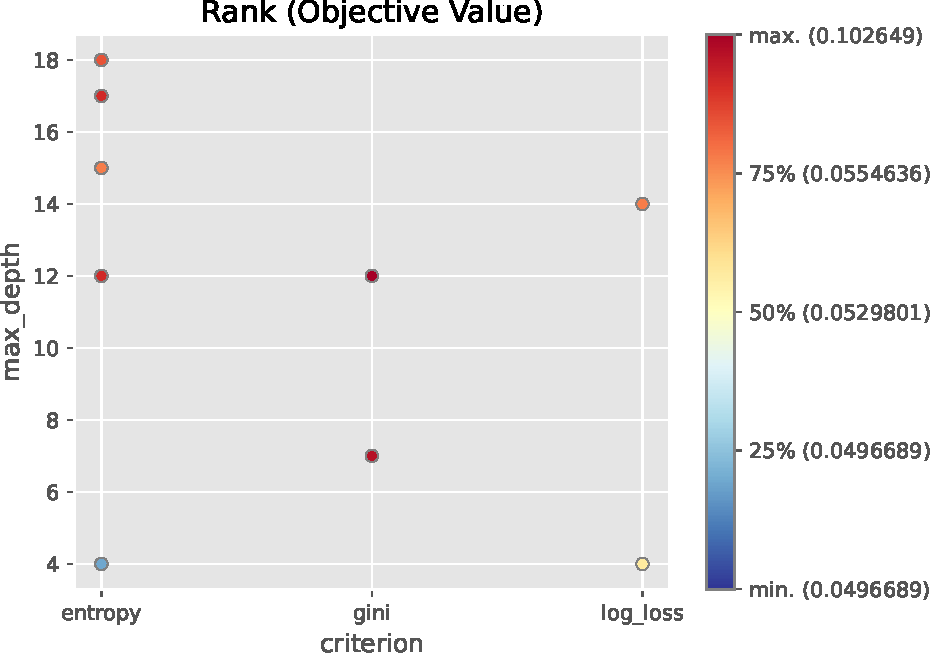
\includegraphics[width=\linewidth]{../../python_code/plots/dt/rank.pdf}
    \end{subfigure}
    %
    \begin{subfigure}{.32\textwidth}
        \centering 
        \caption{}
        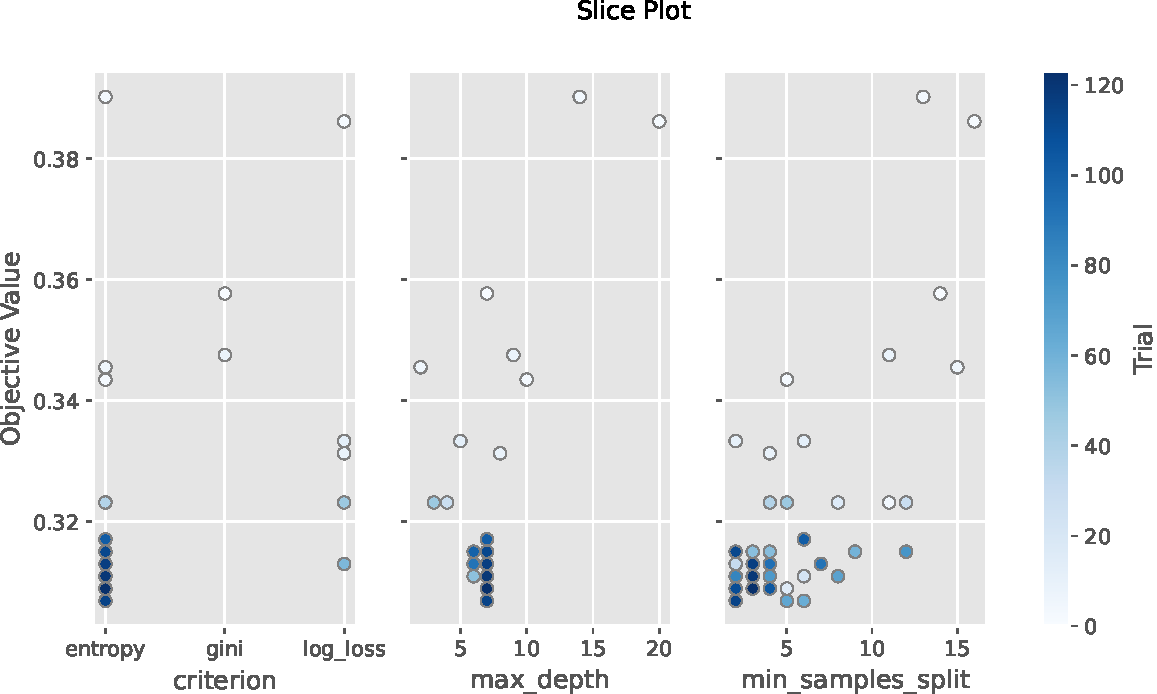
\includegraphics[width=\linewidth]{../../python_code/plots/dt/slice.pdf}
    \end{subfigure}
    \begin{subfigure}{.32\textwidth}
        \centering 
        \caption{}
        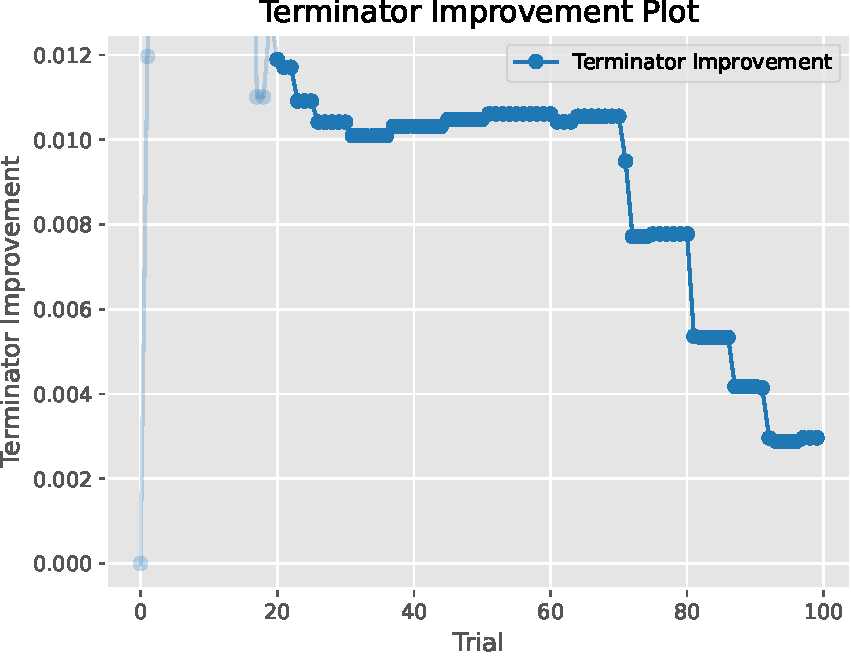
\includegraphics[width=\linewidth]{../../python_code/plots/dt/terminator_improvement.pdf}
    \end{subfigure}
\end{figure}

\clearpage
\subsection{Support Vector Machine}

\begin{figure}[!ht]
    \centering 
    \caption{
        Optuna exploration on SVM hyperparameters. 
        Objective value corresponds to error rate on validation set across all classes.
    }
    \label{fig:optuna_svm}
    \begin{subfigure}{.32\textwidth}
        \centering 
        \caption{}
        
\includegraphics[width=\linewidth]{../../python_code/plots/svm/contour.pdf}
    \end{subfigure}
    \begin{subfigure}{.32\textwidth}
        \centering 
        \caption{}
        
\includegraphics[width=\linewidth]{../../python_code/plots/svm/optimization_history.pdf}
    \end{subfigure}
    %
    \begin{subfigure}{.32\textwidth}
        \centering 
        \caption{}
        
\includegraphics[width=\linewidth]{../../python_code/plots/svm/param_importances.pdf}
    \end{subfigure}
    \begin{subfigure}{.32\textwidth}
        \centering 
        \caption{}
        
\includegraphics[width=\linewidth]{../../python_code/plots/svm/rank.pdf}
    \end{subfigure}
    %
    \begin{subfigure}{.32\textwidth}
        \centering 
        \caption{}
        
\includegraphics[width=\linewidth]{../../python_code/plots/svm/slice.pdf}
    \end{subfigure}
    \begin{subfigure}{.32\textwidth}
        \centering 
        \caption{}
        
\includegraphics[width=\linewidth]{../../python_code/plots/svm/terminator_improvement.pdf}
    \end{subfigure}
\end{figure}